\section{Introduction}

Data centers are responsible for driving large-scale web applications such as web search, storage, advertising, and social network composition ~\cite{chen_understanding_2009, alizadeh_data_2010}. These applications generate diverse traffic patterns with strict throughput and latency requirements. In particular, many distributed web applications rely on a workflow patterns in which requests are broken down and distributed to multiple workers, which perform tasks simultaneously and return responses to an aggregator ~\cite{chen_understanding_2009, alizadeh_data_2010}. As a result, data centers need to support bursts of many-to-one traffic traversing shared bottlenecks without affecting the throughput of long-lived flows needed to update and maintain application data ~\cite{alizadeh_data_2010}.

In order to accommodate the workload generated by these applications while maintaining cost efficiency, modern data centers typically feature high speed links with very low propagation delays, connecting nodes via low-cost switches with shallow buffers ~\cite{chen_understanding_2009, hamilton_designing_2007, alizadeh_data_2010}. The majority of communication between nodes is over TCP, which was designed based on the characteristics of wide area networks, where round-trip times (RTTs) are orders of magnitude greater than in data centers ~\cite{chen_understanding_2009}. As a result, while traditional TCP congestion control mechanisms which are usually considered ``good enough'' in the context of the internet, TCP does not perform well when faced with traffic patterns typical of data center networks ~\cite{chen_understanding_2009, phanishayee_measurement_2008}. 

In particular, the traffic patterns common to data center networks suffer a number of impairments due to problems with traditional TCP congestion control mechanisms. In the synchronized many-to-one scenarios common to distributed applications, TCP connections experience throughput collapse, or incast congestion. In this scenario, good-put at the receiver drops dramatically as simultaneous TCP flows from synchronized senders floods the buffer of a bottleneck switch, causing packet loss and large queuing delays ~\cite{chen_understanding_2009, phanishayee_measurement_2008, dean_mapreduce:_2004}.

In addition, long lived background flows tend to keep switch buffers full, leading to increased queuing delays for latency sensitive traffic. Moreover, improving resource utilization through dynamic buffer allocation means that long lived flows can even cause buffer pressure that impacts flows traversing other ports on a switch ~\cite{alizadeh_data_2010}. More generally, TCP's loss based congestion control mechanism maintains large queues when switch buffers are large, which means that traffic is subject to large queuing delays even in the absence of packet loss, while packet loss at switches with small buffers is misinterpreted as network congestion leading to under-utilization of network resources ~\cite{cardwell_bbr:_2016}.

This paper discusses a number of approaches to TCP congestion control aimed at improving the performance of TCP in data centers. In particular, Data Center TCP (DCTCP) is discussed in depth, and a number of key findings are reproduced using the Mininet network emulator.

\subsection{Data Center Traffic Patterns}

Distributed applications running in modern data centers are based on the \emph{partition/aggregate} design pattern, in which an application is broken in into hierarchical layers and time-sensitive requests at higher layers are divided and delegated to workers in the lower layers. Many workers perform a small component of a task and return a response to an aggregator, which is combined with responses from other workers and passed back up through the hierarchy. An aggregator combines these responses to get a result, which can then be used to send results back to the user. This model is the basis of many data processing frameworks, cluster storage, and targeted advertising applications \cite{chen_understanding_2009, dean_mapreduce:_2004, alizadeh_data_2010}. Requests are often highly time sensitive, with delays at lower levels impacting overall response time and quality \cite{alizadeh_data_2010}.

The traffic supporting supporting applications can be roughly characterized into \emph{query traffic}, \emph{short message trafic}, and \emph{background traffic}.

\subsection{Performance Impairments}

\subsubsection{Incast}

TCP throughput collapse, or TCP \emph{incast},  

\subsubsection{Queue Build-Up}

\subsubsection{Buffer Pressure}

\subsubsection{Buffer Bloat and Underflow}

More generally, traditional loss-based congestion control mechanisms tend to fill buffers, only reducing the TCP send window once packet loss is experienced. This means that large buffers are kept consistently full, resulting in long queuing delays even in the absence of packet loss. Conversely,  

\section{Improving TCP for Data Centers}

\subsection{Incast TCP}

\subsection{Multipath TCP}

\subsection{TCP BBR}

TCP BBR (Bottleneck, Bandwidth, and Round-trip propagation time) uses ``congestion-based congestion control'' in place of traditional loss-based congestion detection mechanisms to improve the performance of TCP. TCP BBR is intended as a general replacement for traditional TCP congestion control mechanisms, though it is currently being implemented in a number of Google services including the Google Cloud Platform as well as Google's B4 Backbone, which is a wide area network comprised of shallow buffered commodity switches similar to those used in data centers ~\cite{cardwell_bbr:_2016, cardwell_tcp_2017}. 

\subsection{Data Center TCP}

Data center TCP (DCTCP) attempts to address the problem of latency in partition/aggregate traffic by reducing queue length without affecting throughput for large TCP flows.

\section{Reproducing Key DCTCP Results}

\subsection{Methods and Results}

Selected results from \cite{alizadeh_data_2010} were reproduced using the Mininet network emulator running on Ubuntu 12.04 with a patched version of the 3.2.18 Linux kernel patched to add in support for DCTCP. While the original study used link speeds of 1 Gbps and 10 Gbps, initial tests showed Mininet was unable to maintain consistent throughput above 150 Mbps even when running on a compute optimized EC2 instance with support for high bandwidth networking (see Limitations). Thus, in order to acheive reliable results, a link speed of 100 Mbps was used in all tests.

\subsubsection{Queue Length}

In order to replicate the queue length results shown in Figures 1 and 13 ~\cite{alizadeh_data_2010}, a simple topology of $N$ flows was constructed with $N$ senders continuously transferring data to a single receiver over a shared bottleneck with a maximum queue length of 400 packets. Figure 1 shows queue length over time for two sustained flows over the shared bottleneck. DCTCP maintained a small steady queue length ($M = 19.38$), while TCP New Reno kept the buffers consistently full with much greater variance in queue length ($M = 330.31$), and exhibited the characteristic sawtooth pattern, with the buffer reaching maximum occupancy at 400 packets before dropping when a loss was detected. Furthermore, Figure 2 shows that DCTCP was much less sensitive to $N$, and maintained consistently low queue sizes at both $N = 2$ and $N = 20$ ($M = 23.63$), whereas queue length for TCP New Reno was consistently greater at $N = 20$ ($M = 368.99$) than when $N = 2$.

\begin{figure}
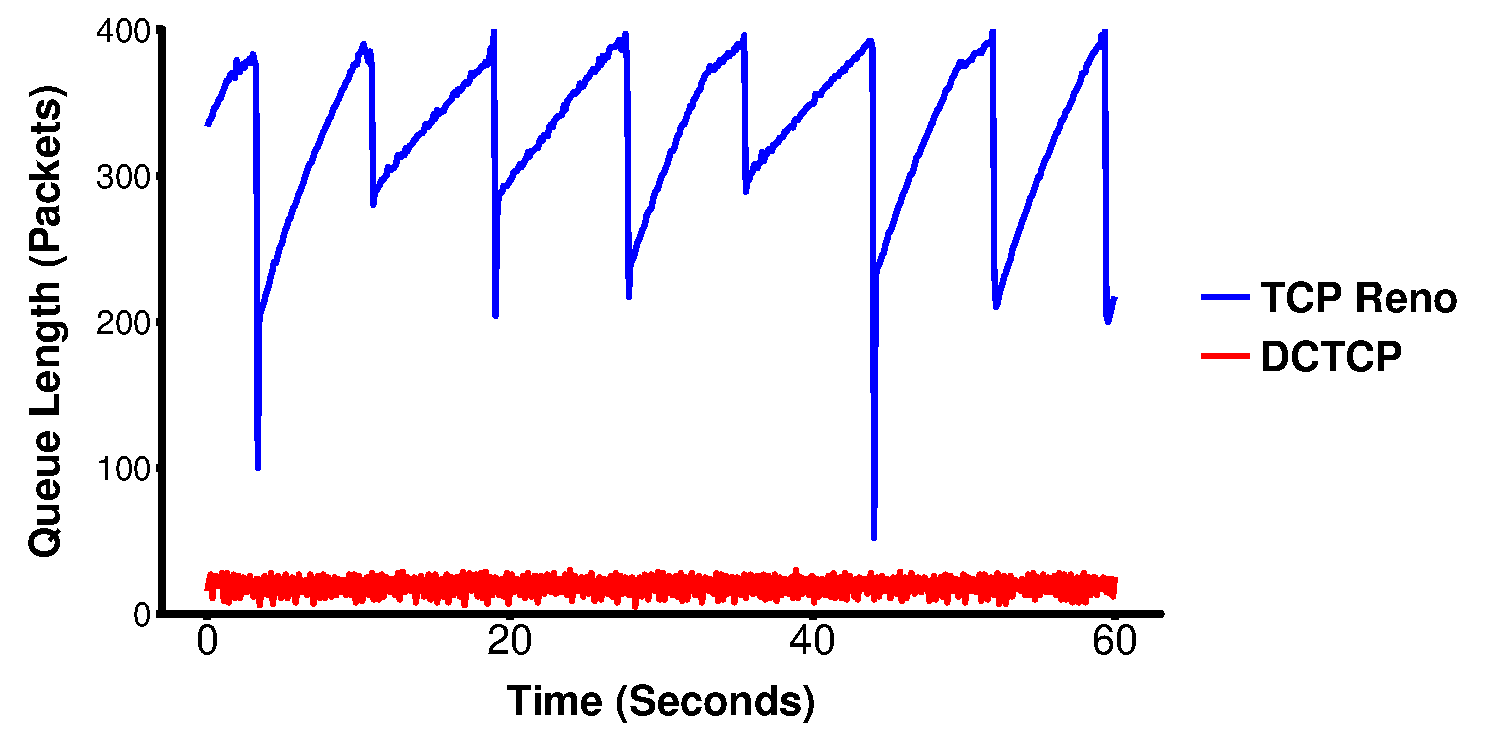
\includegraphics[height=1.75in,width=3.5in]{queue_2_flows}
\caption{Comparison of queue length over time between DCTCP and TCP Reno with 2 flows}
\end{figure}

\begin{figure}
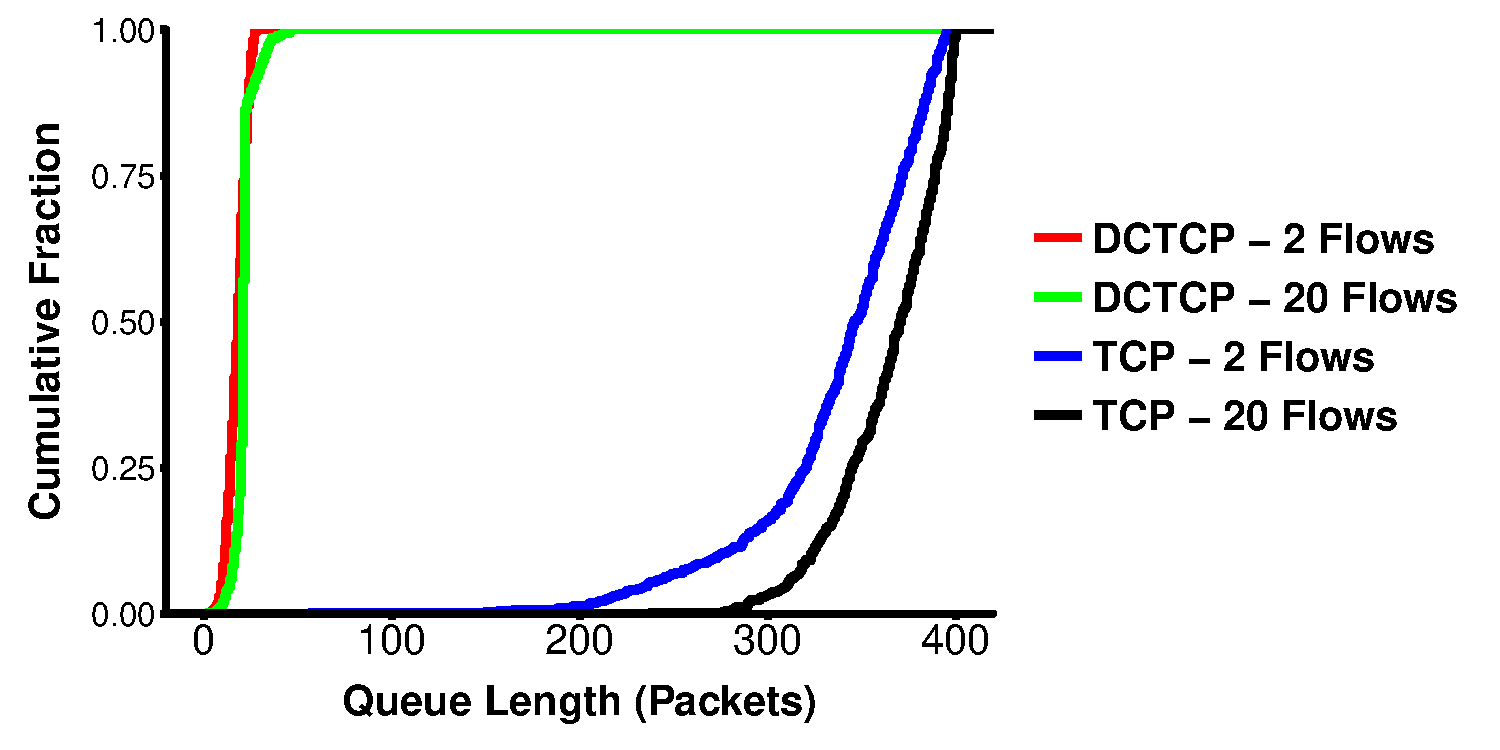
\includegraphics[height=1.75in,width=3.5in]{queue_cdf}
\caption{CDF of queue length for DCTCP and TCP Reno with 2 and 20 flows}
\end{figure}

\subsubsection{Throughput}

Both DCTCP and TCP New Reno made nearly full use of the 100 Mbps bandwidth, maintaining an average of 98.56 and 98.39 Mbps throughput respectively for $N = 2$, which is consistent with the results of the original paper \cite{alizadeh_data_2010}. Additionally, Figure 3 shows the total throughput of two flows transferring data to a single receiver as a function of the marking threshold, $K$. As in the original paper, throughput increased with $K$ until the maximum throughput was reached at $K \approx 20$. The model presented by the authors suggests setting $K$ as a function of link speed and RTT, such that $K > (C \times RTT) / 7$, where C is the link speed in packets/second. An initial test with an RTT of 100$\mu$s and a link speed of 100 Mbps are consistent the authors' findings that throughput is insensitive to $K$ for link speeds of 1 Gbps. Therefore, in order to validate the mathematical model, the RTT was increased to 1 ms since bandwidth was limited to 100 Mbps.

\begin{figure}
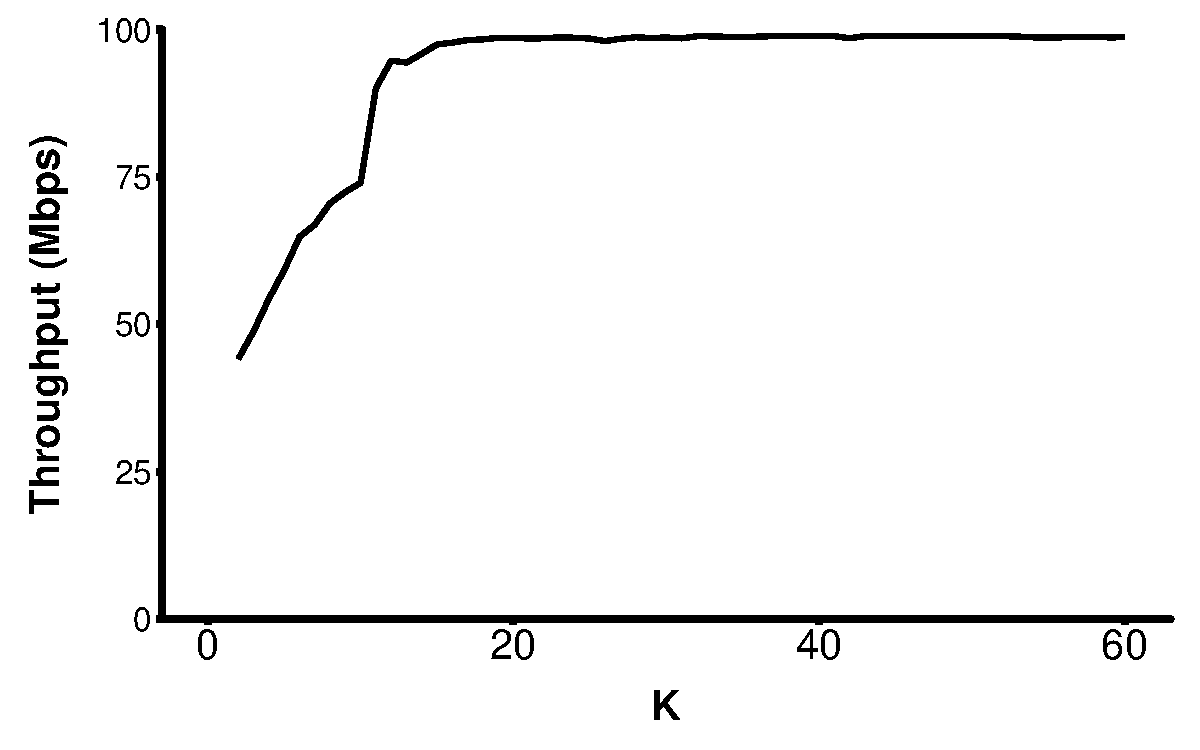
\includegraphics[height=1.75in,width=3in]{k_throughput}
\caption{Throughput as a function of K}
\end{figure}

\subsubsection{Convergence}

Convergence was tested by incrementally starting 5 flows transmitting to a single receiver across a shared bottleneck and allowing each to run for 60 seconds before adding the next flow. Once the fifth flow had run for 60 seconds, each of the 5 flows was stopped in 60 second intervals. The results of the DCTCP convergence test (Figure 4) show that each of the DCTCP flows quickly converges to its fair share of the available bandwidth with little variability. In addition, the total bandwidth across the flows indicated consistently high throughput as flows were started and stopped.

Interestingly, the results of the TCP New Reno convergence test showed considerably more variability.  

\begin{figure}
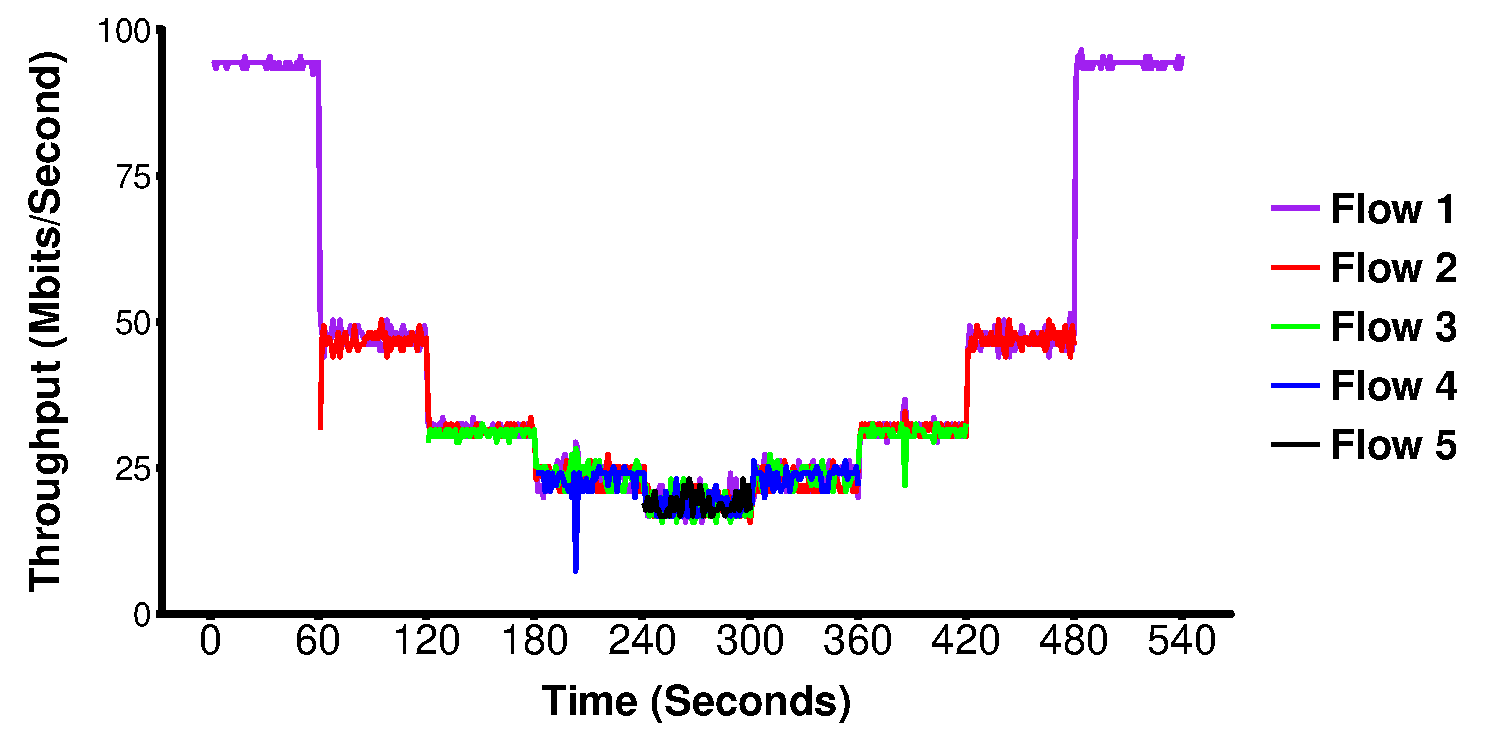
\includegraphics[height=1.75in,width=3.5in]{dctcp_converg}
\caption{Convergence of 5 flows DCTCP}
\end{figure}

\begin{figure}
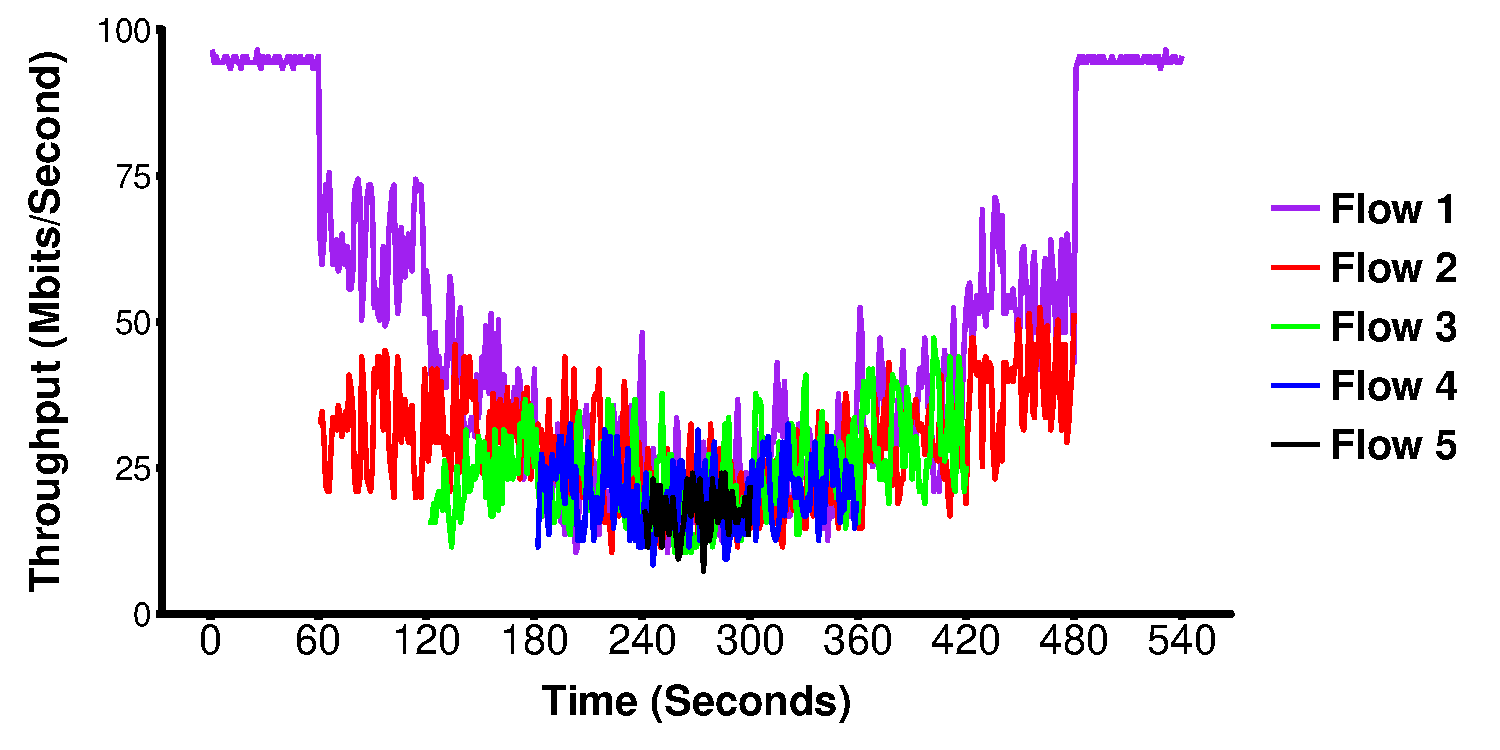
\includegraphics[height=1.75in,width=3.5in]{reno_converg}
\caption{Convergence of 5 flows TCP Reno}
\end{figure}

\subsection{Limitations}

\section{Conclusions}

